\section{Expanded Model}

\begin{frame}{Motivation}
\begin{itemize}
  \item previous model: phenotypic distance tied directly to fitness score
  \item add more sophisticated fitness evaluation to separate phenotypic distance and fitness score
  \item adjust genetic regulatory network setup to scale better   \item add hidden states to allow greater network intricacy
\end{itemize}
\end{frame}

\begin{frame}{Conway's Game of Life}
\begin{figure}
  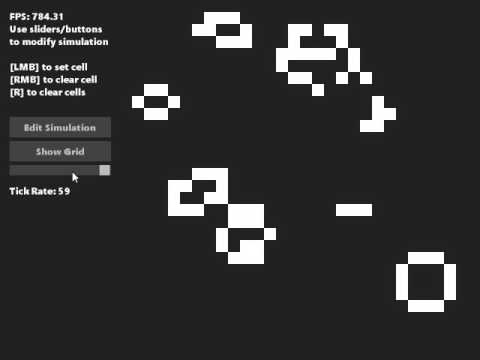
\includegraphics[width=0.8\textwidth]{img/gol_icon}
  \captionsetup{singlelinecheck=off,justification=raggedright}
\href{https://www.youtube.com/watch?v=Kzg5is1lgSk}{\caption{Video illustrations of Conway's Game of Life cellular automata in action.}}
\end{figure}
\end{frame}

\begin{frame}{Adjusted Genetic Regulatory Network Model}
\begin{figure}
    \centering
    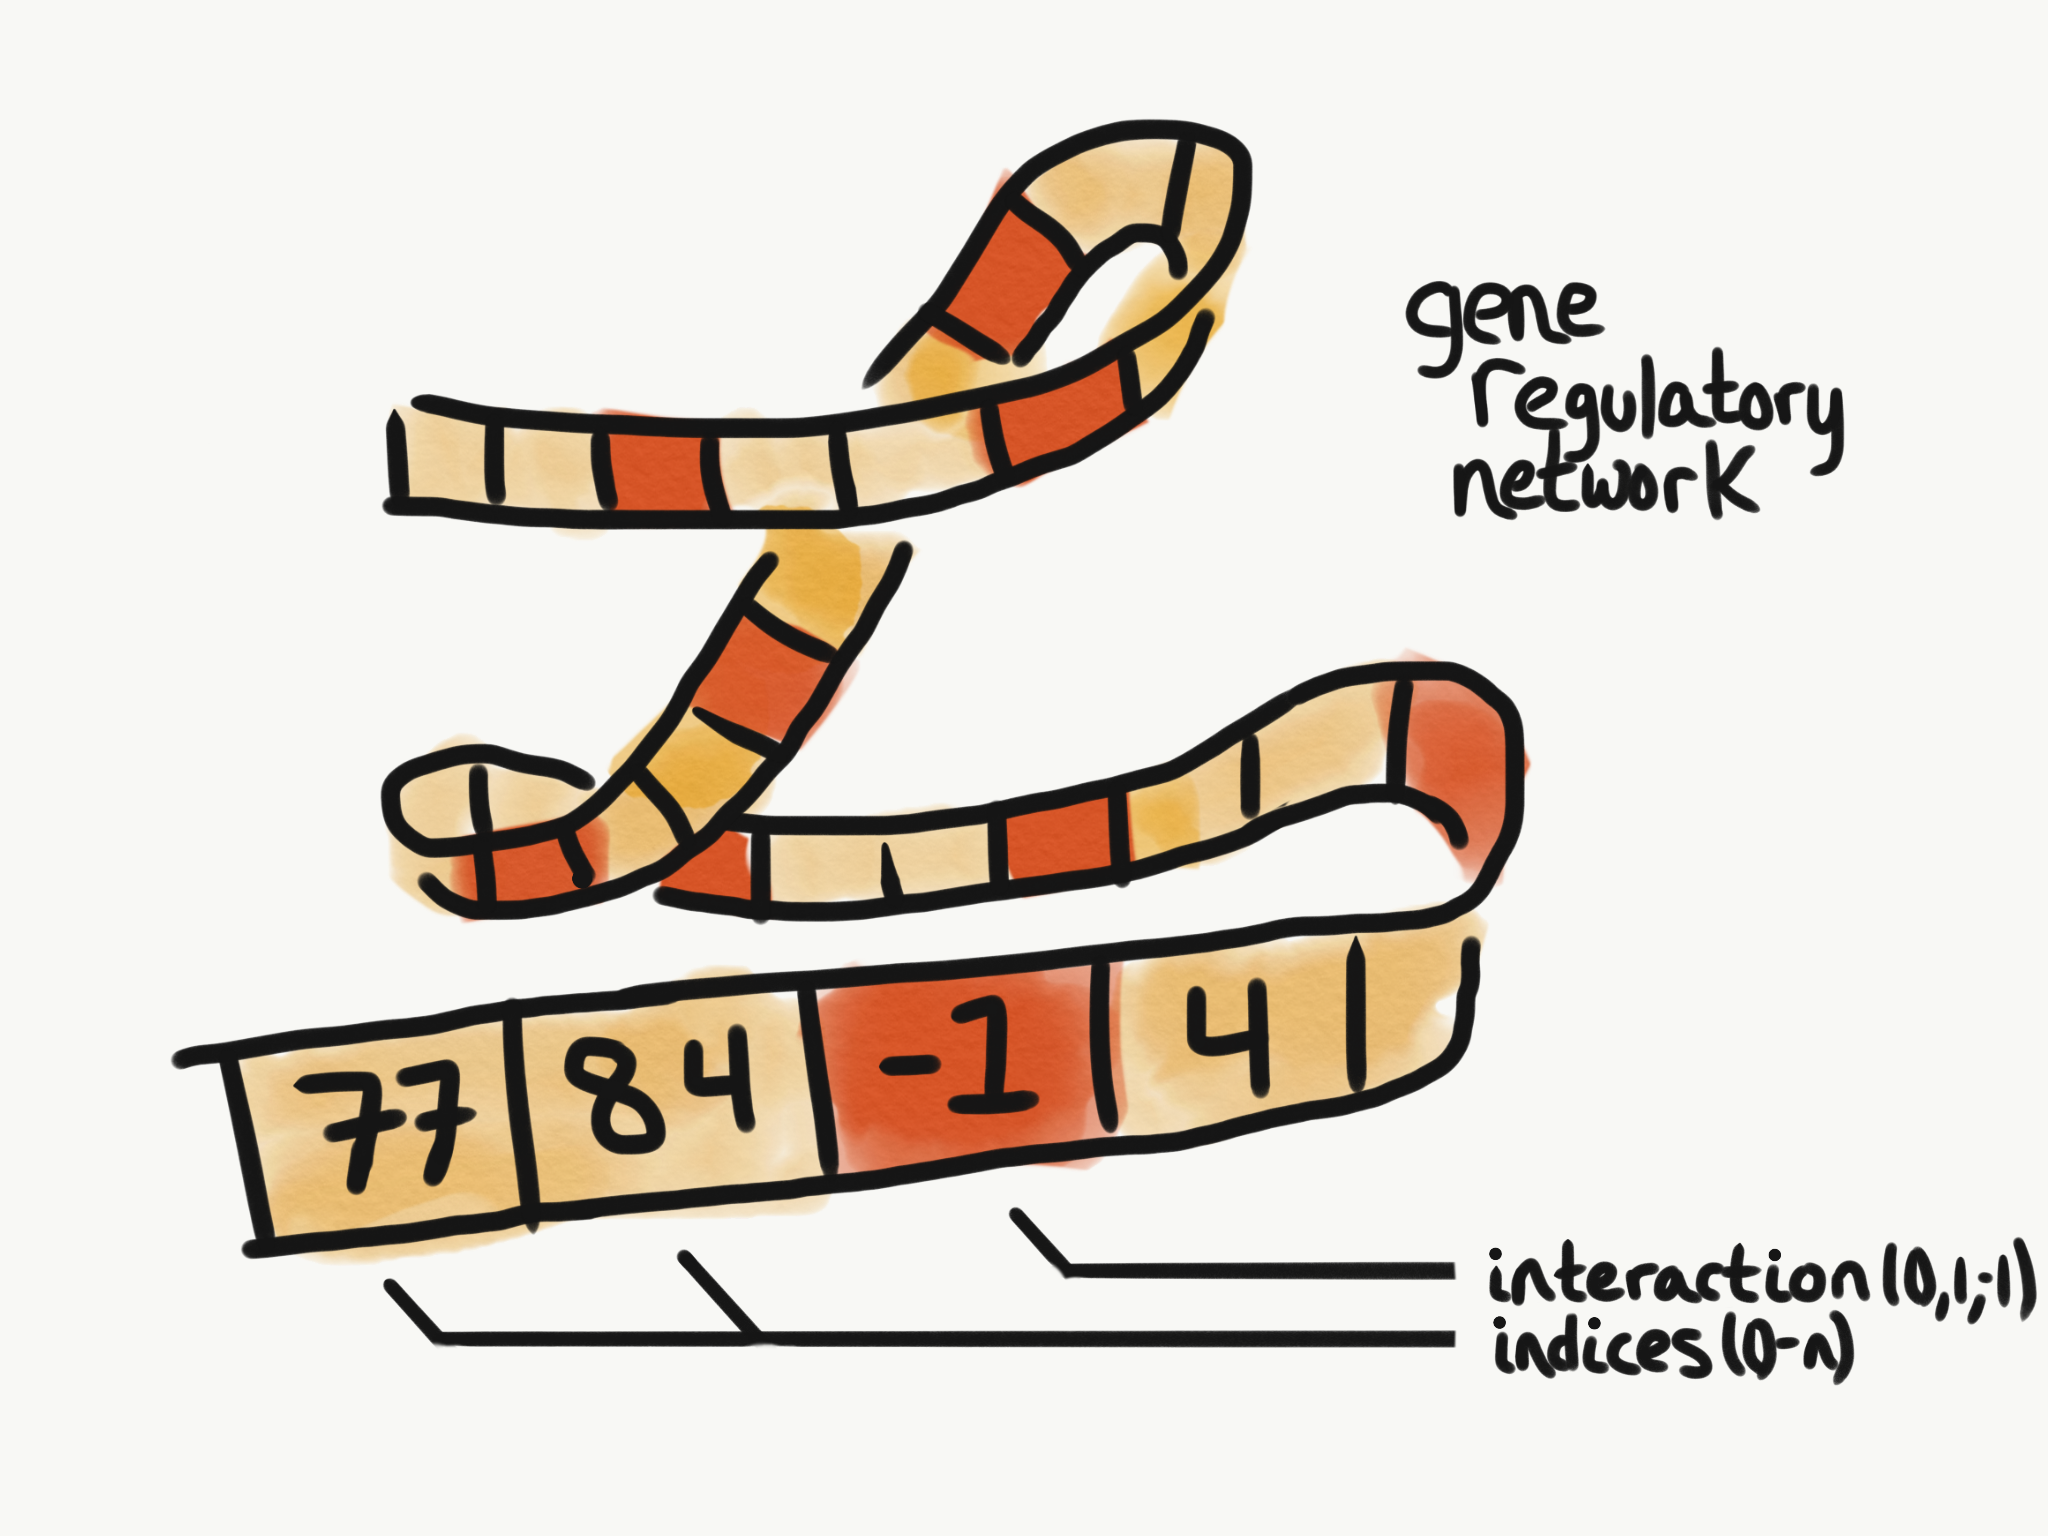
\includegraphics[width=0.8\textwidth]{img/expanded_grn}
 	\captionsetup{singlelinecheck=off,justification=raggedright}
  	\caption{A cartoon depiction of the expanded genetic regulatory network model employed, originally inspired by \cite{Wilder2015ReconcilingEvolvability}.}
    \label{fig:expanded_grn}
\end{figure}
\end{frame}

\begin{frame}{Complete Model}
\begin{figure}
    \centering
    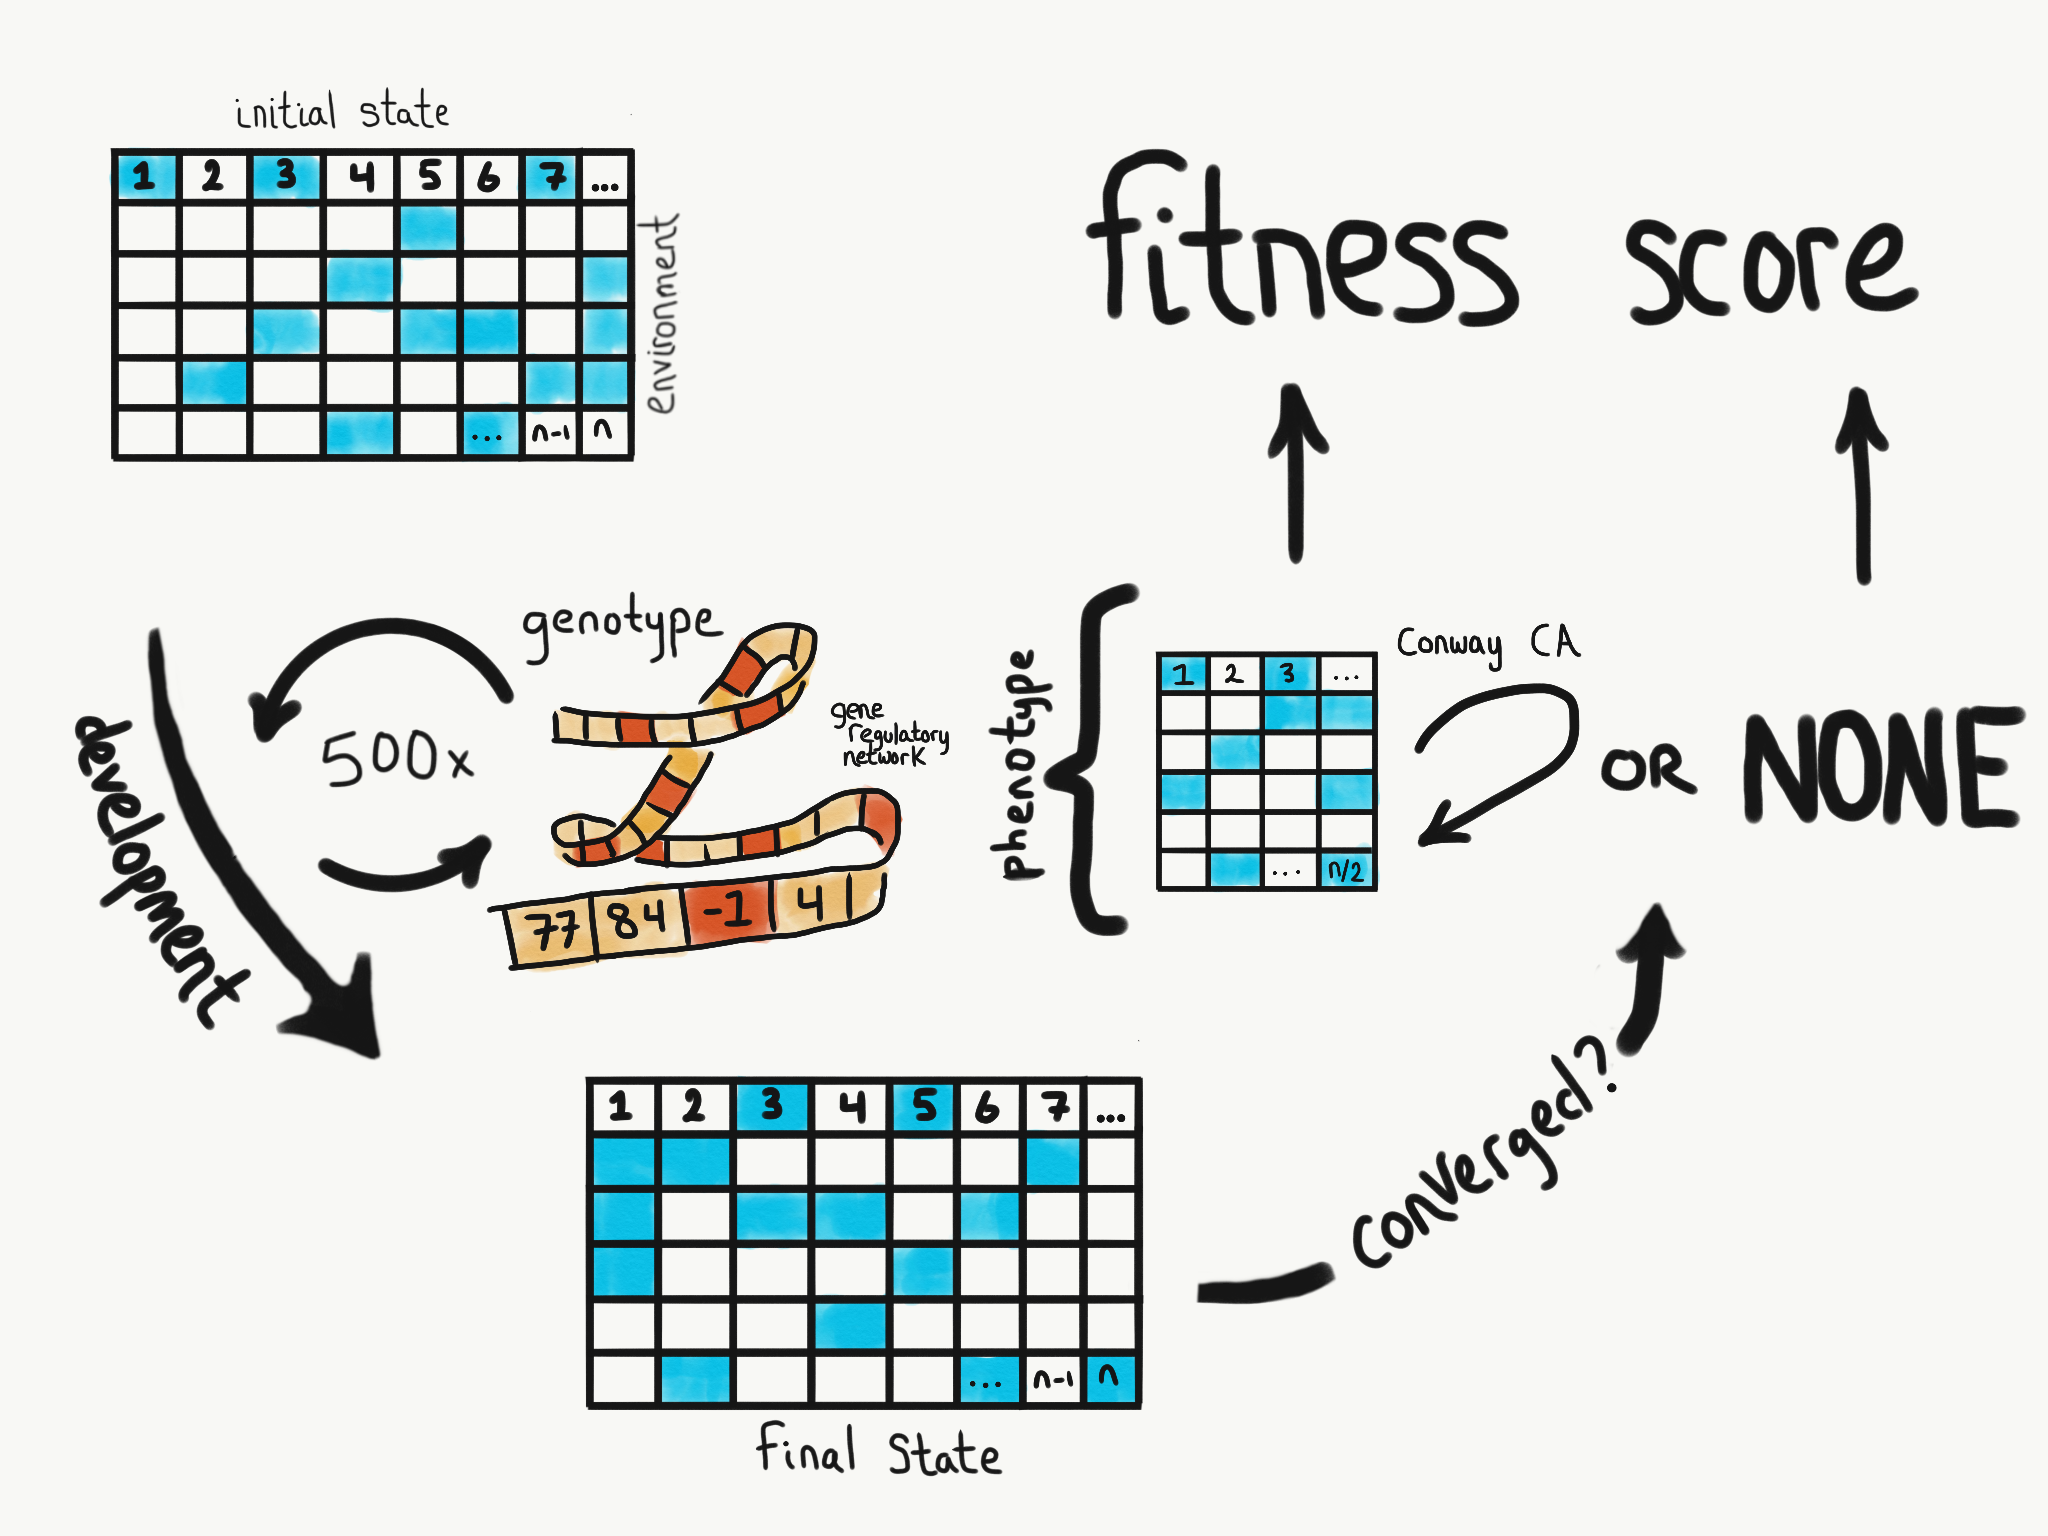
\includegraphics[width=0.8\textwidth]{img/complete_schematic}
 	\captionsetup{singlelinecheck=off,justification=raggedright}
  	\caption{A cartoon overview of the development and assessment processes of the expanded model, based loosely on \cite{Wilder2015ReconcilingEvolvability}.}
    \label{fig:complete_schematic}
\end{figure}
\end{frame}

\begin{frame}{Direct Plasticity: Initial State Perturbation}
\begin{figure}
    \centering
    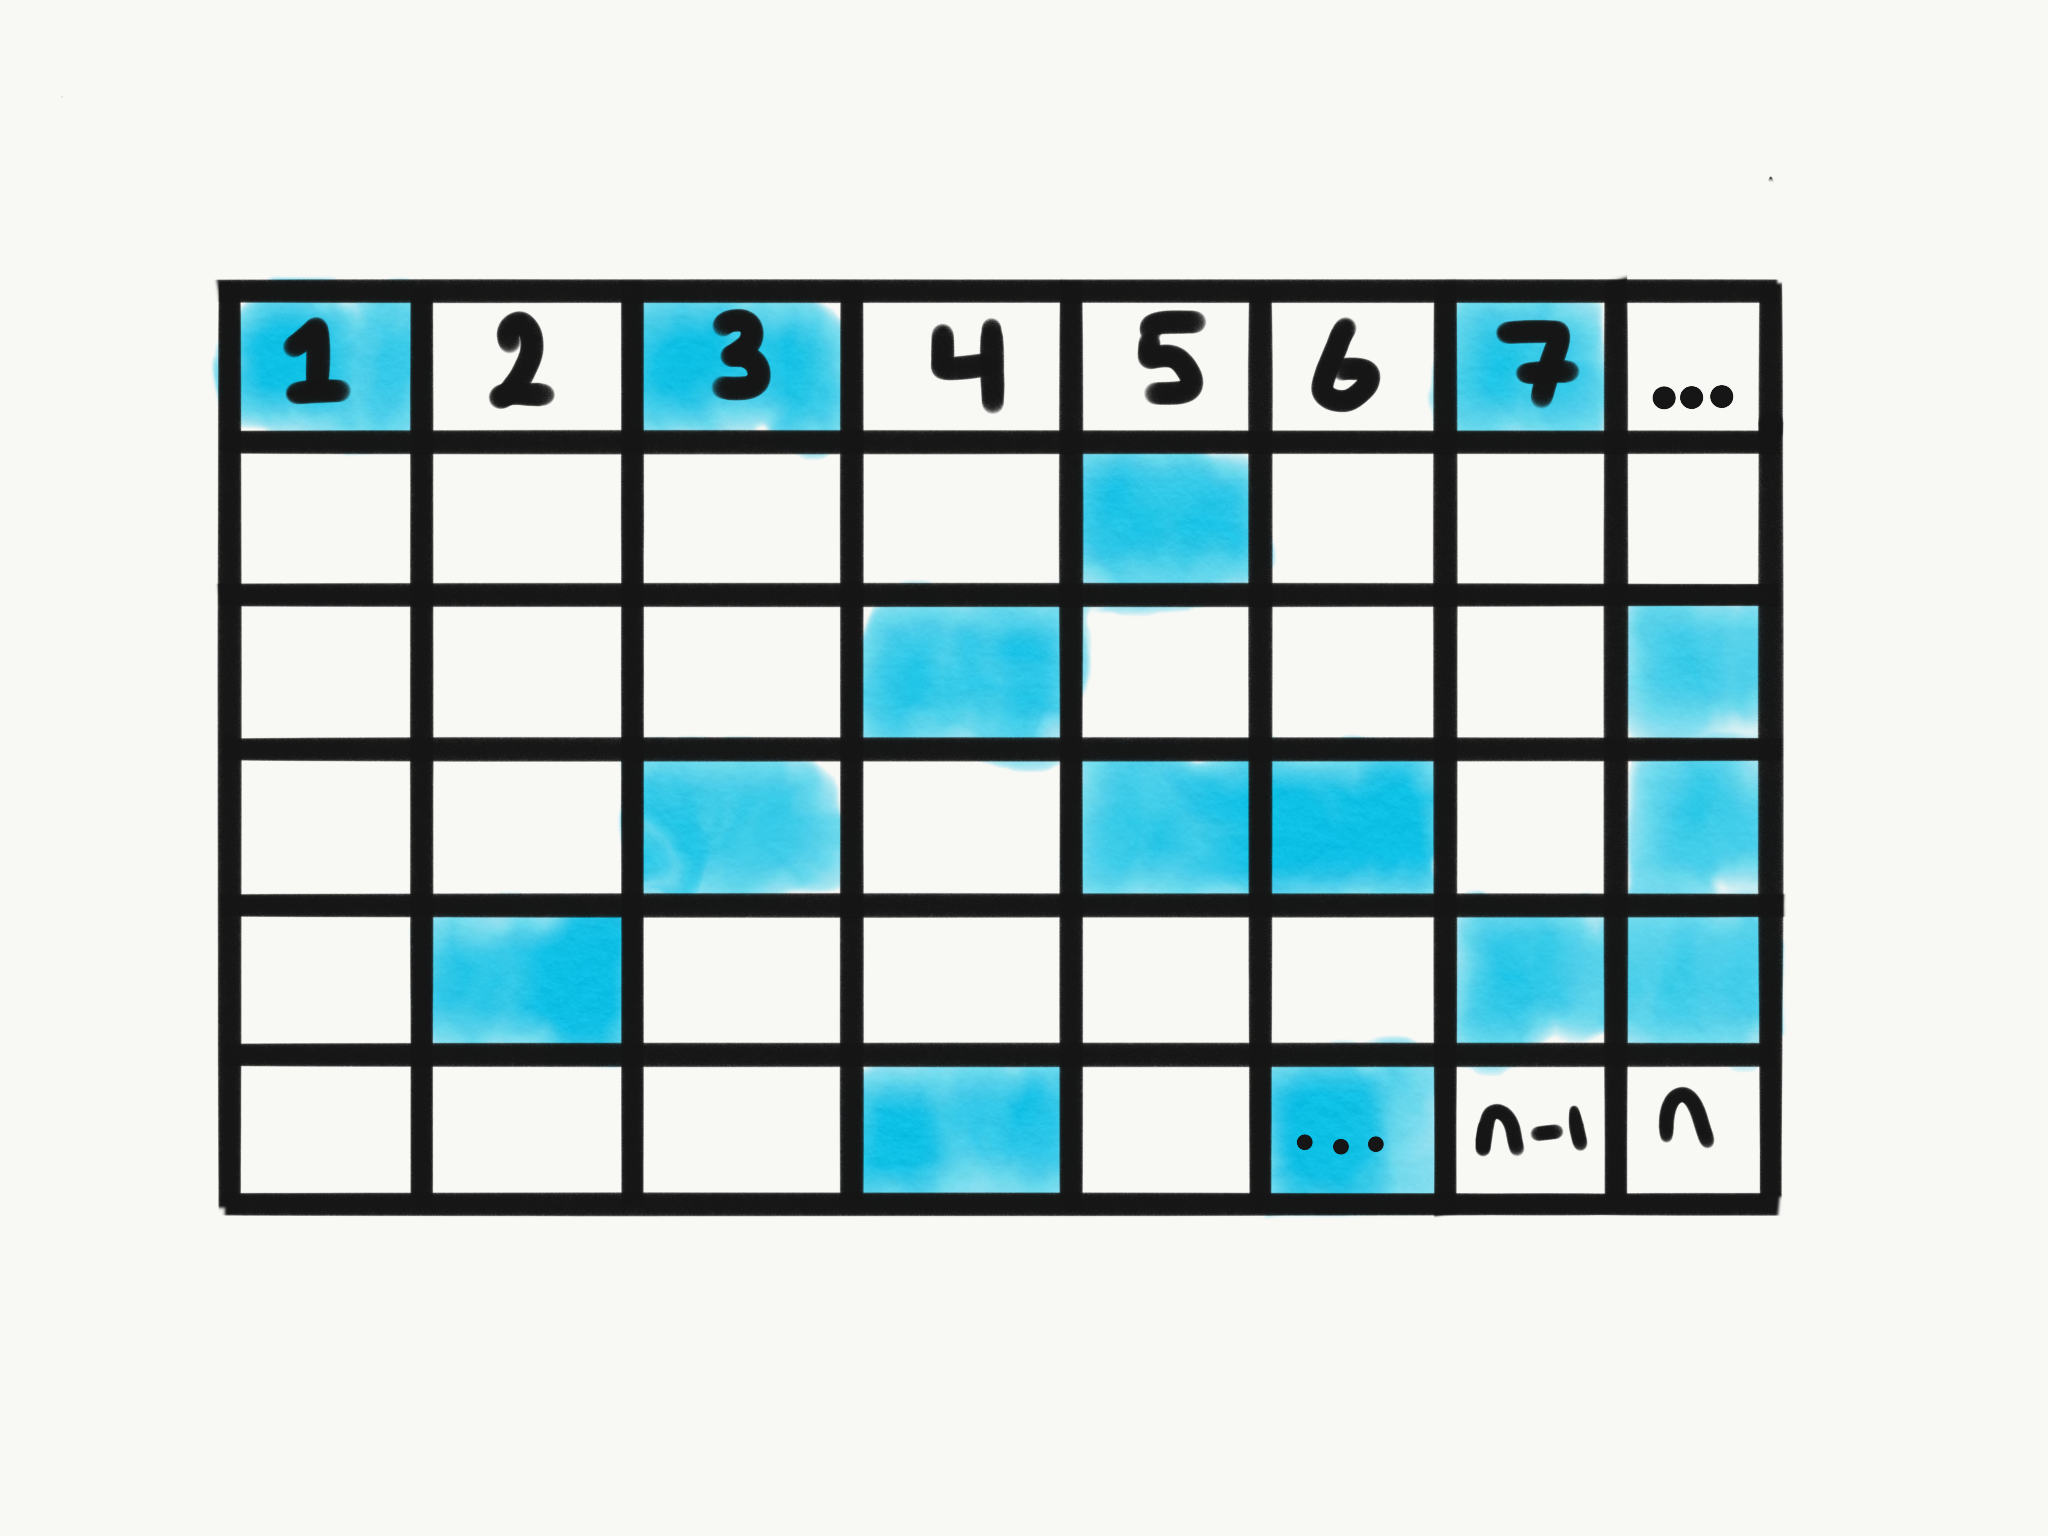
\includegraphics[width=0.8\textwidth]{img/initial_state}
 	\captionsetup{singlelinecheck=off,justification=raggedright}
  	\caption{A graphical example of an initial state, which represents environmental conditions encountered by the genetic regulatory network.}
    \label{fig:initial_state}
\end{figure}
\end{frame}

\begin{frame}{Direct Plasticity: Initial State Perturbation}
\begin{figure}
    \centering
    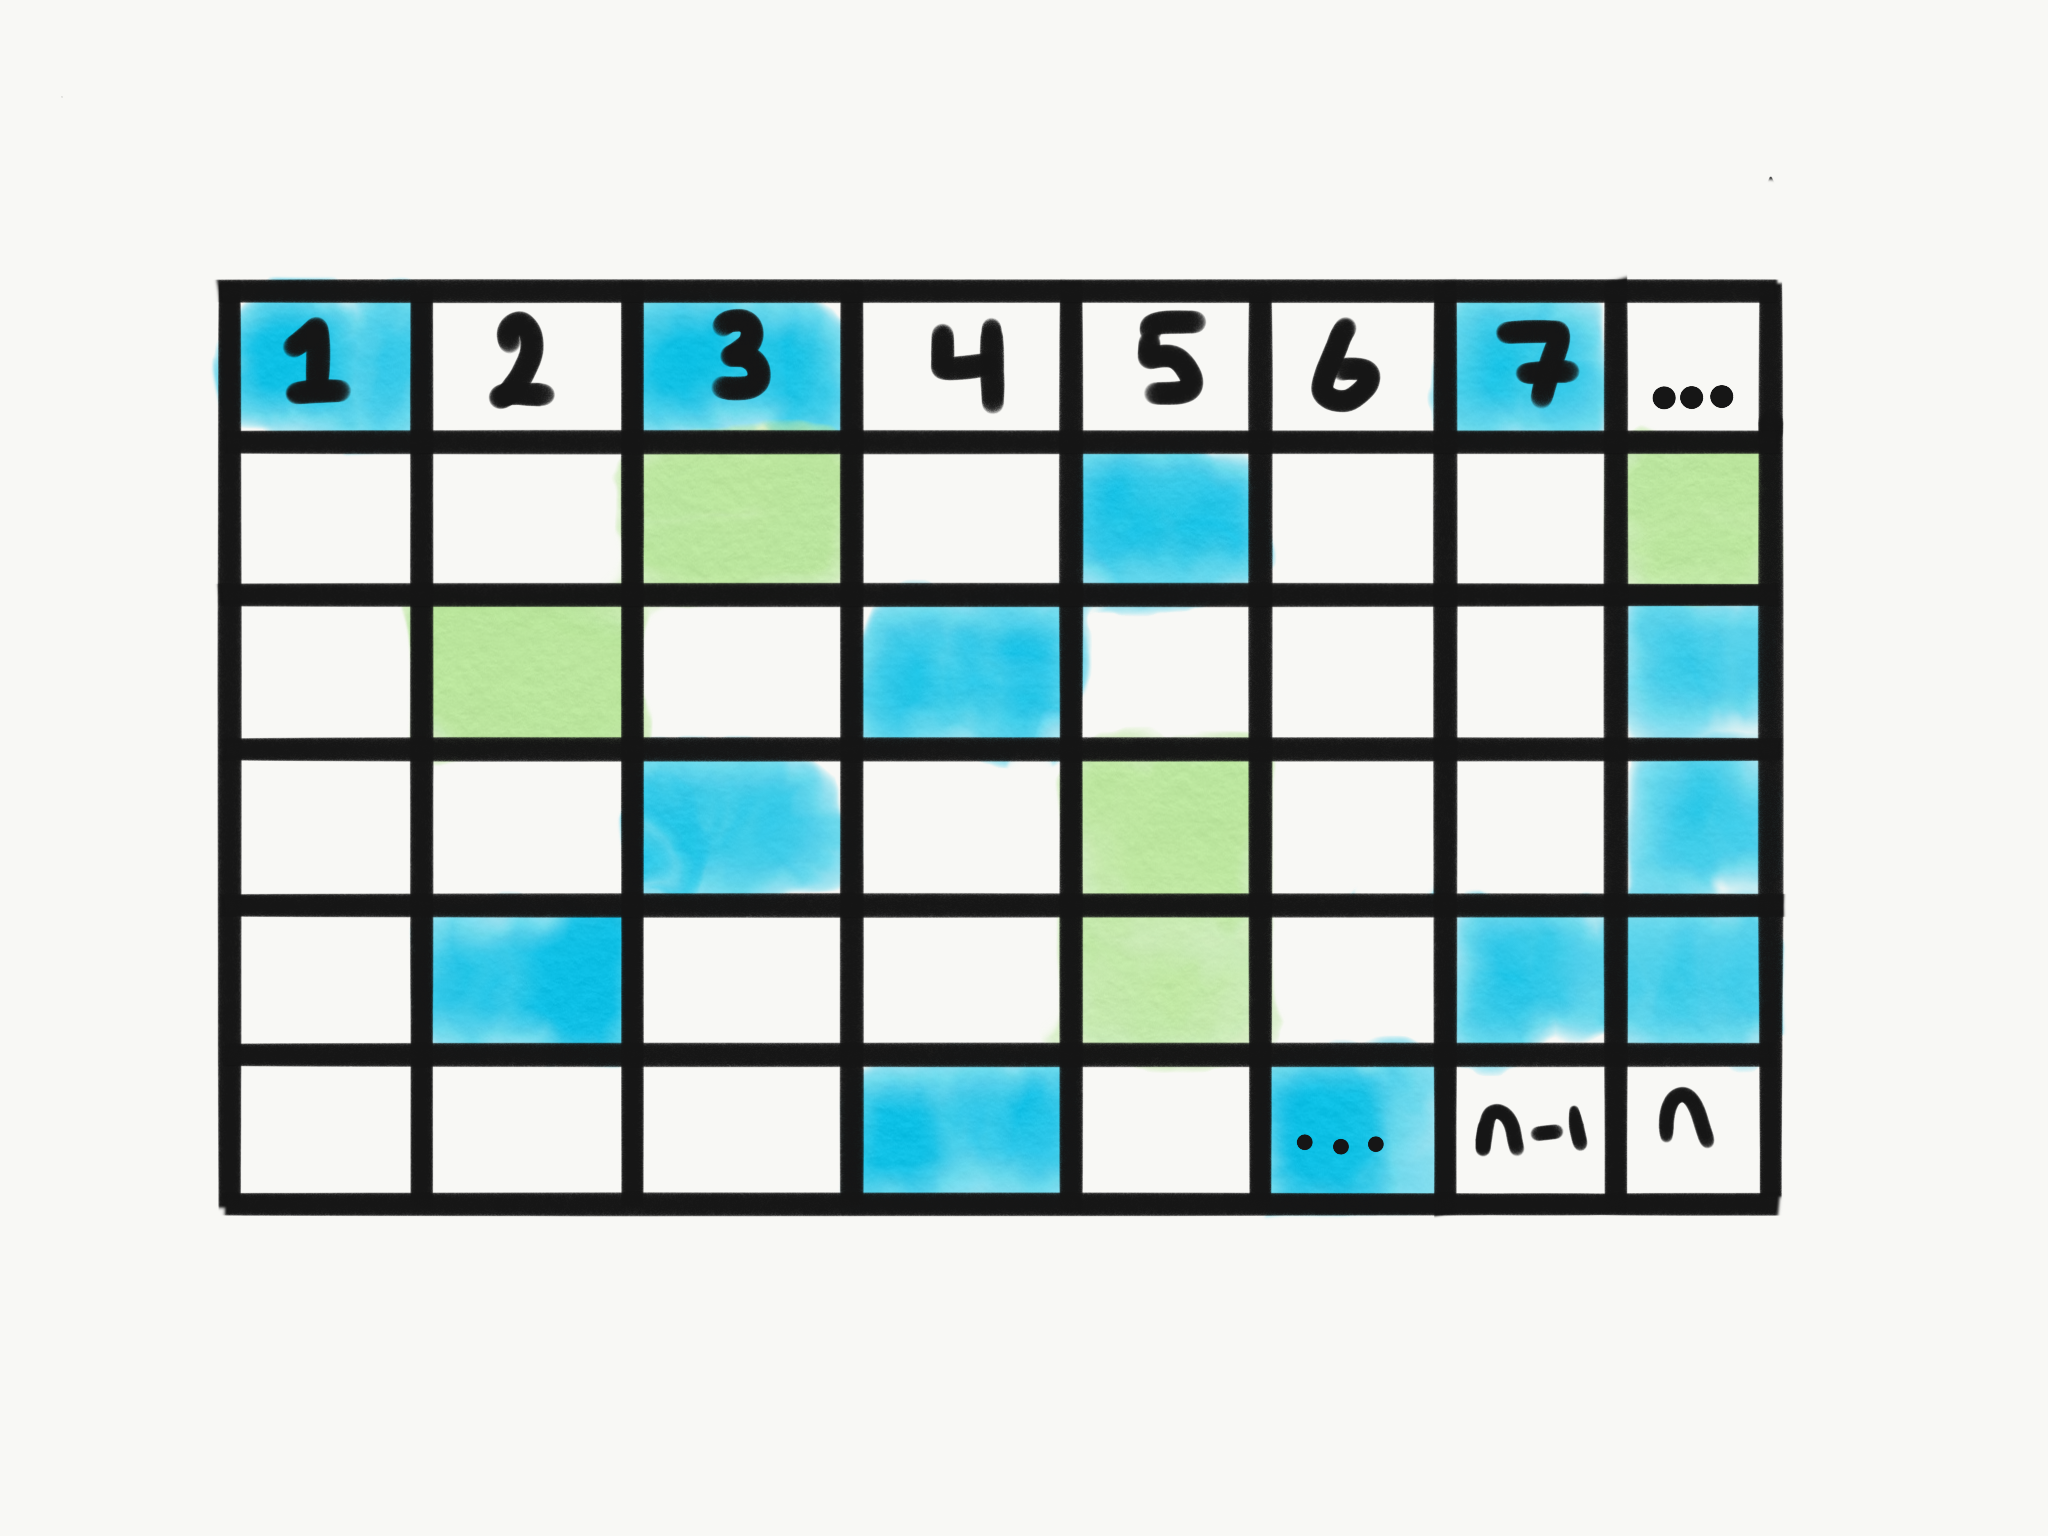
\includegraphics[width=0.8\textwidth]{img/perturbed_initial_state}
 	\captionsetup{singlelinecheck=off,justification=raggedright}
  	\caption{A graphical example of an initial state after random perturbation.}
    \label{fig:perturbed_initial_state}
\end{figure}
\end{frame}

\begin{frame}{Direct Plasticity: Initial State Perturbation}
\begin{figure}
    \centering
    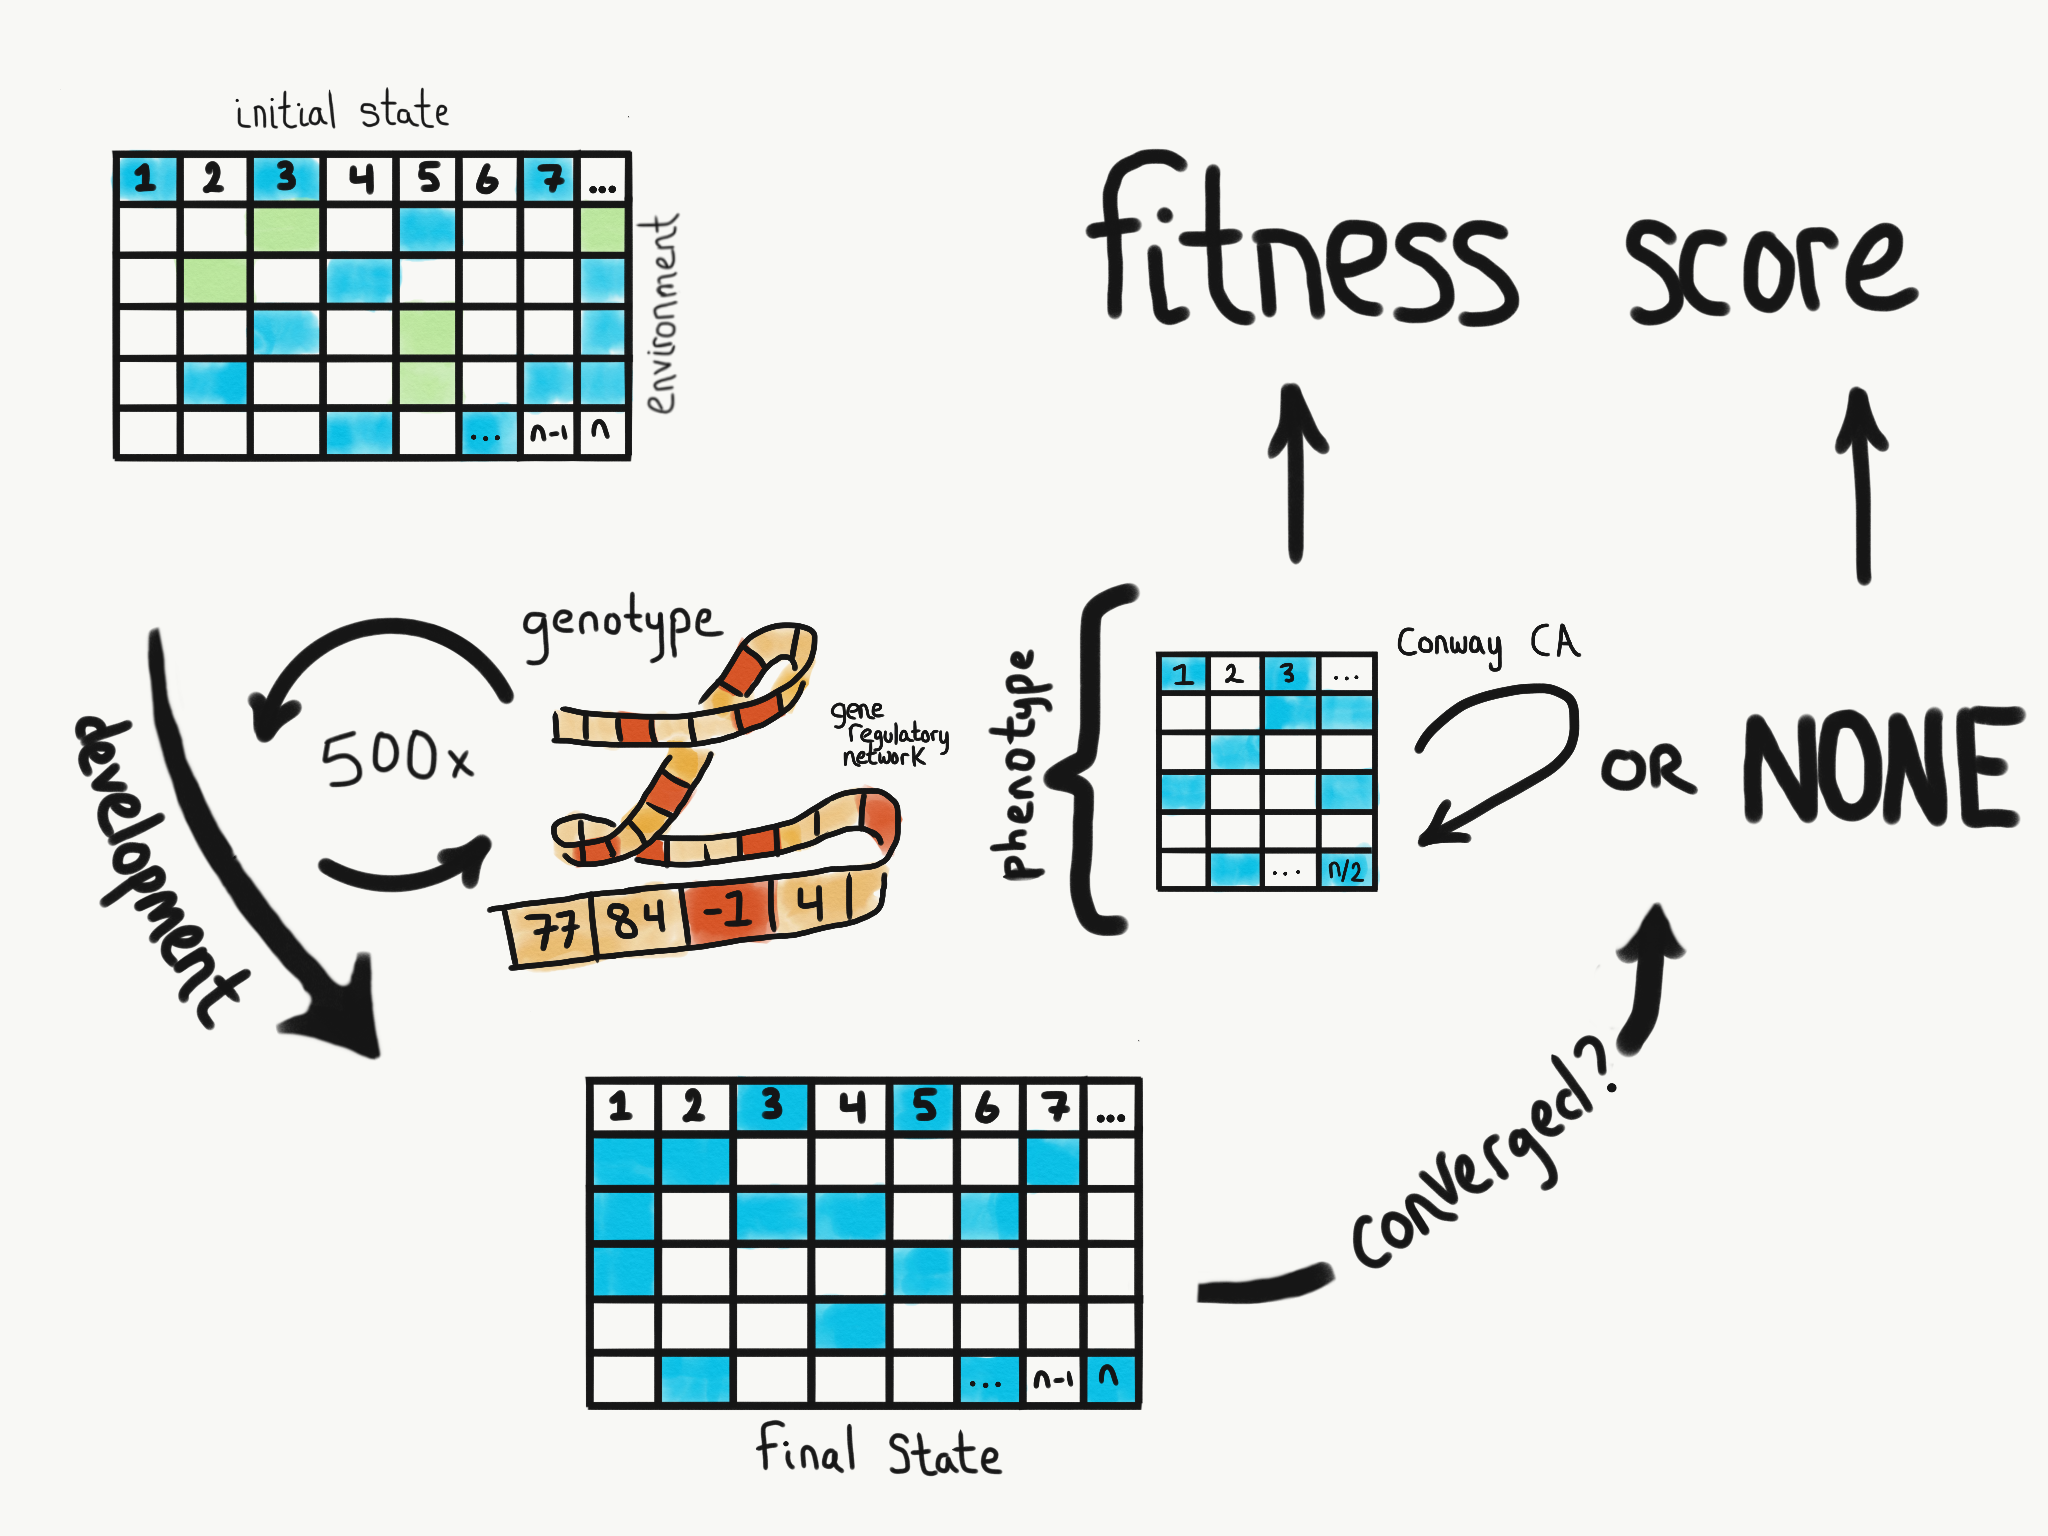
\includegraphics[width=0.8\textwidth]{img/complete_schematic_perturbed}
 	\captionsetup{singlelinecheck=off,justification=raggedright}
  	\caption{A cartoon overview of the development and assessment processes of the expanded model depicting perturbed initial conditions.}
    \label{fig:complete_schematic}
\end{figure}
\end{frame}

